\RequirePackage{ifpdf}
\ifpdf
   \documentclass[a4paper,11pt,pdftex,twoside]{scrartcl}
\else
   \documentclass[a4paper,11pt,dvips,twoside]{scrartcl}
\fi

% ------------------------------------------------------------------------------
% Include packages
% ------------------------------------------------------------------------------
\ifpdf
   \usepackage[pdftex]{color}
   \usepackage[final,pdftex]{graphicx} % Einbinden von Gaphiken, flexibler als package {graphics}
\else
   \usepackage[dvips]{color}
   \usepackage[final,dvips]{graphicx}
\fi
\usepackage[german]{babel}   % Deutsche Übersetzung, Trennung...
\usepackage[utf8]{inputenc}  % Ermöglicht die Verwendung von UTF8 Zeichensätzen 
                             % und damit der direkten Eingabe von Sonderzeichen, d.h. z.B. Umlaute.
\usepackage[T1]{fontenc}
\usepackage{caption}
\usepackage{url}
\usepackage{tabularx}
\usepackage{booktabs}
\usepackage{longtable}
\usepackage[table]{xcolor}
\usepackage{xspace}   % 
\usepackage{float}
\usepackage{lscape}
%\usepackage[square]{natbib}
\usepackage{amsmath}
\usepackage{amsfonts}
\usepackage{amssymb}
\usepackage{upgreek}
%\usepackage{longtable}
\usepackage{placeins}
\usepackage{subfigure}
\usepackage{amsthm}
\usepackage{hyperref}

\newtheorem*{definition}{Definition}



% PAGE LAYOUT
\setlength{\topmargin}{0.2cm}
\setlength{\headheight}{0cm}
\setlength{\headsep}{0cm}

\setlength{\textheight}{\paperheight}
\addtolength{\textheight}{-2.2in}

\setlength{\oddsidemargin}{0.1cm}
\setlength{\evensidemargin}{\oddsidemargin}
\setlength{\textwidth}{\paperwidth}
\addtolength{\textwidth}{-2in}
\addtolength{\textwidth}{-1.8\oddsidemargin}

% new commands
\newcommand{\superscript}[1]{\ensuremath{^{\textrm{#1}}}}
\newcommand{\subscript}[1]{\ensuremath{_{\textrm{#1}}}}

\renewcommand{\th}[0]{\superscript{th}}
\newcommand{\st}[0]{\superscript{st}}
\newcommand{\nd}[0]{\superscript{nd}}
\newcommand{\rd}[0]{\superscript{rd}}

\newcommand{\celsius}{$^{\circ}\mathrm{C}$}
\newcommand{\degree}{$^{\circ}$}

% Color defintions
\definecolor{gray1}{rgb}{0.95,0.95,0.95}
\definecolor{gray2}{rgb}{0.85,0.85,0.85}

%
\newcommand{\comment}[1]{\textcolor{red}{>>[\TODO] #1<<}}


\newcommand{\ethz}{\emph{ETH Zürich}\xspace}
\newcommand{\iwf}{\emph{Institut für Werkzeugmaschinen und Fertigung (IWF), \ethz}\xspace}
\newcommand{\inspire}{\emph{inspire AG}\xspace}
\newcommand{\eclipseprojectplace}{\href{http://www.eclipse.org/downloads/}{Projektseite}\xspace}

\newcommand{\appref}[1]{Anhang \ref{#1}}
\newcommand{\secref}[1]{Abschnitt \ref{#1}}
%\newcommand{\equref}[1]{Equation \ref{#1}} %better use builtin \eqref{} !!!
\newcommand{\figref}[1]{Abbildung \ref{#1}}
\newcommand{\tabref}[1]{Tabelle \ref{#1}}

\renewcommand{\comment}[1]{\textcolor{red}{\textbf{**TODO**} #1}}

\newcommand{\iwfadmin}{Administrator (\href{mailto:meile@iwf.mavt.ethz.ch}{J. Meile})\xspace}
\newcommand{\developper}{Entwickler (\href{mailto:hampl@iwf.mavt.ethz.ch}{D. Hampl}, \href{mailto:sizuest@inspire.ethz.ch}{S. Züst})\xspace}

\bibliographystyle{alpha}

% ============================================================================
% Define Titlepage
% ============================================================================
\subject{Energiemodell (EMod)}
\title{Setup und erste Schritte}
\subtitle{Version: 0.1\\(Draft)}
\author{S. Züst}
\date{\today}
%\publishers{\vspace{20mm}}  % Abused to separate title from abstract
\titlehead{
    \vspace{-15mm} 
    \hspace{-3mm}
    \begin{tabular}{lp{3cm}l}
        
\includegraphics[width=65mm]{logos/eth_logo.jpg} &&
        
\includegraphics[width=45mm]{logos/inspire_logo.jpg}\\
    \end{tabular}
    \vspace{10mm} 
    \hspace{0mm}

}
\publishers{}
% ============================================================================

\begin{document}

% ----------------------------------------------------------------------------
% Make titlepage
% ----------------------------------------------------------------------------
\maketitle
\thispagestyle{empty} % No headers, no page numbers

\clearpage

\thispagestyle{empty} % No headers, no page numbers
\tableofcontents
\clearpage

%\pagestyle{plain} % No headers, just page numbers
\pagenumbering{arabic} % Roman numerals
\setcounter{page}{1}   % Start page numbering

% ----------------------------------------------------------------------------
% Einleitung
% ----------------------------------------------------------------------------
\section{Einleitung}
Für die Modellierung und Simulation der Ressourcenflüssen auf Produktionsmaschinen ist am \iwf zusammen mit \inspire das Framework \emph{EMod} (Energiemodell) in Entwicklung.
Das fertige Tool soll ermöglichen, bereits in der frühen Planungsphase erste Aussagen über den Energie- und Ressourcenverbrauch auf Komponentenebene zu machen.
Dabei wird der Anwender in der Modellbildung durch eine Modellbibliothek und Parameterdatenbank unterstützt.
Die Modellbibliothek beinhaltet Markomodelle von einzelnen Komponententypen.
Solche Makromodelle beinhalten ein definiertes Interface aus physikalischen und logischen Ein- und Ausgängen, sowie eine Beschreibung der Dynamik zwischen diesen Ein- und Ausgängen.
Diese Makromodelle werden anhand einer Parameterdatenbank konfiguriert. 
Dabei entspricht ein Eintrag in der Parameterdatenbank einem spezifischen Komponententyp (z.B Synchronmotor des Herstellers X vom Typ Y).
Der Anwender des Frameworks kann nun ein Modell seiner Maschine erstellen, indem er die Wirkzusammenhänge zwischen den einzelnen Komponenten vorgibt.
Sobald das Modell erstellt ist, kann die Leistungsaufnahme für ein gegebenes Szenario simulativ berechnet werden.
Das Tool ist schematisch in Abbildung \ref{fig:emod} dargestellt.

\begin{figure}[h]
	\centering
	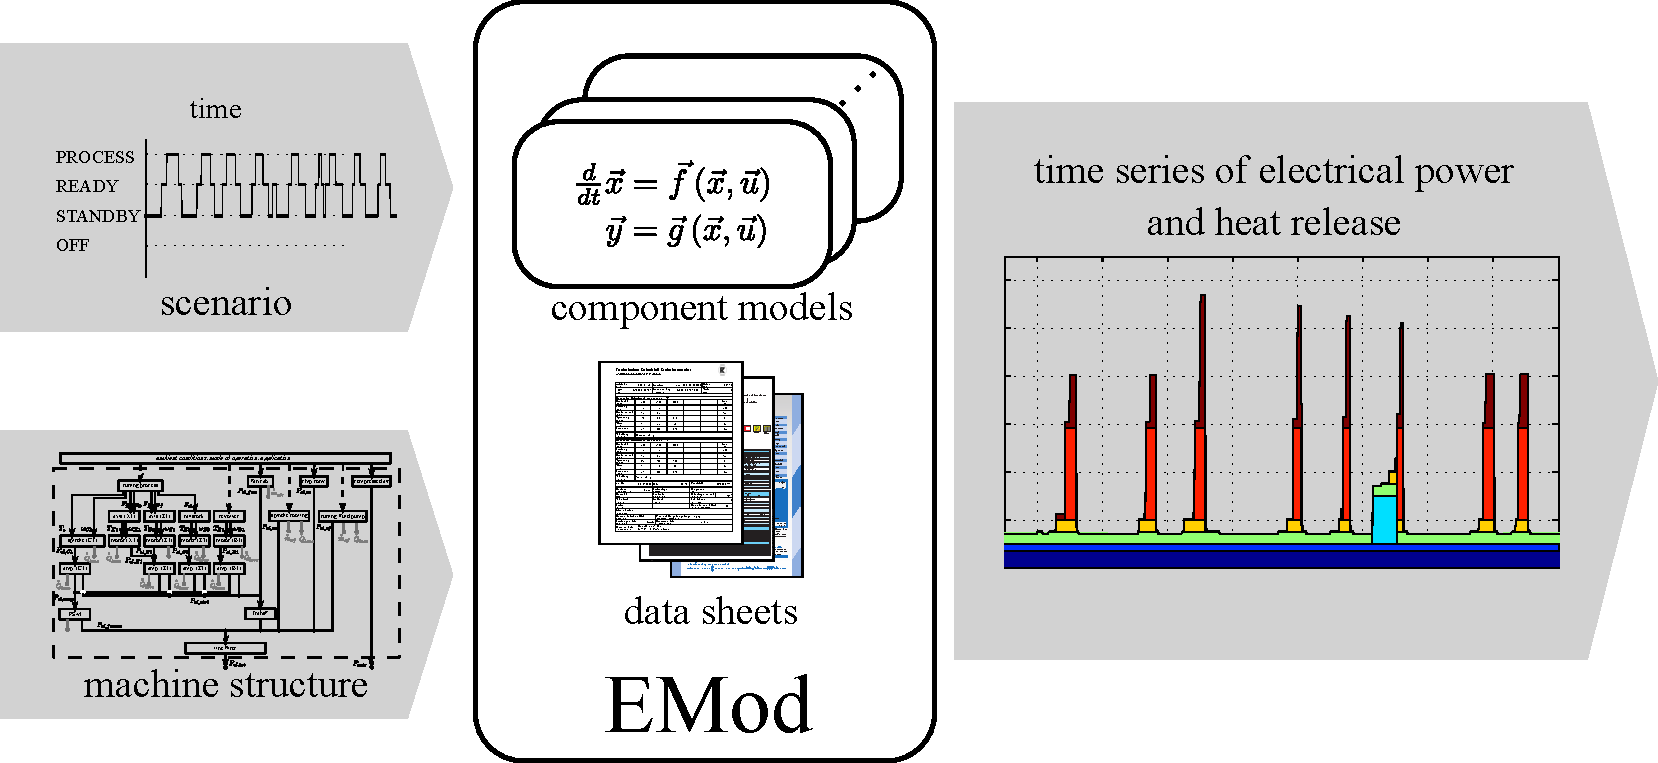
\includegraphics[width=.8\linewidth]{figures/emod}
	\caption{Schematische Darstellung des Simulationsframeworks \emph{Energiemodell} (WZM).}
	\label{fig:emod}
\end{figure}

Das Framework wird in \emph{Java} entwickelt.
Um den Einstieg für neue Entwickler am \iwf oder \inspire zu erleichtern, beinhaltet das vorliegende Dokument alle Informationen über die benötigte Software, sowie die notwendigen Arbeitsschritte.
Weiter werden Richtlinien und erwartete Arbeitsweisen vorgestellt.

% +++++++++++++++++++++++++++++++++++++++++++++++++++++++++++++++++++++++++++
% SETUP
% +++++++++++++++++++++++++++++++++++++++++++++++++++++++++++++++++++++++++++
\section{Setup}
Dieses Kapitel beschreibt die notwendigen Schritte um mit dem Entwicklungsbeitrag an \emph{EMod} starten zu können.
Als erstes wird die verwendete Entwicklungssoftware beschrieben.
Anschliessend erfolgt die Datenbeschaffung, sowie die initiale Konfiguration.

% ===========================================================================
% SOFTWARE
% ===========================================================================
\subsection{Software}
Im wesentlichen werden drei Softwaretools für die Entwicklung eingesetzt: 
Eclipse, Subversion und Redmine.
Die Beschaffung dieser Software ist in den nachfolgenden Abschnitten beschrieben.
Für weitere Informationen zu den einzelnen Softwaren, sowie deren Bedienung sei auf die entsprechenden Dokumentationen verwiesen.

% ---------------------------------------------------------------------------
% Eclipse
% ---------------------------------------------------------------------------
\subsubsection{Eclipse}
%\begin{quotation}
%	\emph{Eclipse (von englisch eclipse „Sonnenfinsternis“, „Finsternis“, „Verdunkelung“) ist ein quelloffenes Programmierwerkzeug zur Entwicklung von Software verschiedenster Art. Ursprünglich wurde Eclipse als integrierte Entwicklungsumgebung (IDE) für die Programmiersprache Java genutzt, aber mittlerweile wird es wegen seiner Erweiterbarkeit auch für viele andere Entwicklungsaufgaben eingesetzt. Für Eclipse gibt es eine Vielzahl sowohl quelloffener als auch kommerzieller Erweiterungen.
%Eclipse selbst basiert auf Java-Technik, seit Version 3.0 auf einem sogenannten OSGi-Framework namens Equinox.} [\href{http://de.wikipedia.org/wiki/Eclipse_\%28IDE\%29}{Wikipedia} ]
%\end{quotation}

Für die Entwicklung und Pflege des Softwarecodes wird  \emph{Eclipse} empfohlen.
Die Software kann von der \eclipseprojectplace sowohl für Windows, Linux und Mac OS X bezogen werden.
Für die Installation sind die Einleitungen auf der \eclipseprojectplace zu berücksichtigen.
Falls Eclipse das erste mal eingesetzt wird, empfiehlt sich das Tutorial \emph{Hello World}: \texttt{Help} $\rightarrow$ \texttt{Cheat sheets...} $\rightarrow$ \texttt{Java Development} $\rightarrow$ \texttt{Create a hello World [SWT] application}.

% ---------------------------------------------------------------------------
% Eclipse
% ---------------------------------------------------------------------------
\subsubsection{SWT}
\comment{Link \& Installationsanleitung}
Das \emph{Standart Widget Toolkit (SWT)} wird für die graphische Oberfläche des Tools benötigt.
das Toolkit kann über die \href{http://www.eclipse.org/swt/}{Projektseite} bezogen werden.
Beim Download ist auf die richtige Plattform (Windows, Linus, OS X), sowie die richtige Architektur (23/64 Bit) zu achten.



% ---------------------------------------------------------------------------
% SVN
% ---------------------------------------------------------------------------
\subsubsection{Subversion Client}

%\begin{quotation}
%	\emph{Apache Subversion (SVN) ist eine freie Software zur Versionsverwaltung von Dateien und Verzeichnissen.
%	Die Versionierung erfolgt in einem zentralen Projektarchiv (engl. repository) in Form einer einfachen Revisionszählung.
%	Wenn Änderungen an Inhalten verteilt auf den Computern der Bearbeiter ausgeführt werden, werden zwischen dem Projektarchiv und einem Arbeitsplatz jeweils nur die Unterschiede zu bereits vorhandenen Ständen übertragen.} [\href{http://de.wikipedia.org/wiki/Apache\_Subversion}{Wikipedia} ]
%\end{quotation}

Für das parallele Arbeiten am Projektcode im Team wird \textit{Subversion} (SVN) eingesetzt.
Um Subversion zu nutzen, gibt es abhängig von der Plattform verschiedene Lösungen.
Eine Auswahl ist in Tabelle \ref{tab:svnclients} gegeben:

\begin{table}[h]
	\centering
	\caption{Ausgewählte SVN-Clients für verschiedene Plattformen}\label{tab:svnclients}
	\rowcolors{2}{gray2}{gray1}
	\begin{tabular}{lcccl}
		\textbf{Programm}		& \textbf{Windows}	& \textbf{Linux}	& \textbf{Mac OS X}	& \textbf{Quelle}\\
		\hline
		svn                 &   & $\bullet$ & $\bullet$ & Packetquelle\\
		Tortoise SVN        & $\bullet$ &  $\bullet$ &   & \href{http://tortoisesvn.tigris.org/}{tortoisesvn.tigris.org}\\
		Eclipse Subversive  & $\bullet$ & $\bullet$ & $\bullet$ & \href{http://www.eclipse.org/subversive/}{www.eclipse.org/subversive}\\
		SVN Workbench       &   & $\bullet$ &   & Packetquelle
	\end{tabular}
\end{table}

% ---------------------------------------------------------------------------
% Redmine
% ---------------------------------------------------------------------------
\subsubsection{Redmine}
%

Um das Projekt \emph{EMod} zu verwalten wird \emph{Redmine} eingesetzt. 
Auf Redmine ist der Projektplan mit allen Arbeitspaketen einsehbar.
Weiter können Tickets für Korrektur- oder Verbesserungsvorschläge gelöst werden.
In \emph{Redmine} sind auch die Informationen aus dem SVN-Repository abrufbar.
So können verschiedene Versionen miteinander verglichen werden, oder die Änderungen eines bestimmten Versionsschritts gelesen werden.
Der Zugriff auf \emph{Redmine} erfolgt über einen Browser der Wahl:

\begin{center}
	\href{https://icvrdevil.ethz.ch/redmine/projects/emodid}{https://icvrdevil.ethz.ch/redmine/projects/emodid}
\end{center}
Der Zugang kann beim \iwfadmin oder bei einem \developper beantragt werden.

% ===========================================================================
% CHECKOUT
% ===========================================================================
\subsection{Checkout}
Der Vorgang Checkout beschreibt die Beschaffung der, hier aktuellsten, Version der Daten auf dem Repository.
Dazu empfiehlt es sich wie folgt vorzugehen:
\begin{enumerate}
	\item Neues Verzeichnis erstellen, indem die Daten abgelegt werden sollen (z.B \texttt{~/Dokumente/EMod})
	\item Den Subversion Client entsprechende einrichten. Der Pfad zu Repository ist \\\texttt{https://icvrdevil.ethz.ch/svn/EMod}.
	Der Zugang kann beim \iwfadmin über einen \developper beantragt werden.
	\item Nach der erfolgten Enrichtung des Clients den Checkout durchführen.
	Dabei wird lokal eine Kopie der aktuellen Version auf dem Repository erstellt.
	Details, bzw. das genaue Vorgehen für den Checkout sind der Dokumentation des verwendeten Clients zu entnehmen. 	
	\item Das Projekt kann anschliessend in Eclipse importiert werden. Dazu Eclipse starten und den Entsprechenden Dialog über \emph{File $\rightarrow$ Import ...} öffnen.
	Anschliessend unter \emph{General} die Option \emph{Existing Projects into Workspace} selektieren und mit \emph{Next >} bestätigen.
	Nun ist unter \emph{Select root directory} das Verzeichnis \texttt{trunk/ch.ethz.inspire.emod} in dem unter 1. erstellten Verzeichnis (z.B \texttt{~/Dokumente/EMod}) anzugeben und der Import mit \emph{Finish} abzuschliessen
\end{enumerate}



% ===========================================================================
% KONFIGURATION
% ===========================================================================
\subsection{Konfiguration}

% +++++++++++++++++++++++++++++++++++++++++++++++++++++++++++++++++++++++++++
% ERSTE SCHRITTE
% +++++++++++++++++++++++++++++++++++++++++++++++++++++++++++++++++++++++++++
\section{Erste Schritte}

% ===========================================================================
% PROGRAMSTRUKTUR
% ===========================================================================
\subsection{Programstruktur}

% ===========================================================================
% GUIDELINES
% ===========================================================================
\subsection{Guidelines}


\end{document}
